% Masing-masing dasar teori terdiri dari:
% - What - definisi, contoh
% - Why - alasan digunakan
% - How - Penggunaan dalam tugas akhir

\chapter{TINJAUAN PUSTAKA} \label{chap:tinjauan-pustaka}
\tab Bab ini menjelaskan dasar teori yang digunakan dalam analisis, perancangan, dan implementasi struktur data dan algoritme untuk menjawab permasalahan \textit{k-Most Promising Products} ($k$-MPP) berbasis interval waktu pada data multidimensi dengan serial waktu yang diangkat dalam Tugas Akhir ini. 

\section{Daftar Notasi}
\tab Tabel \ref{tab:daftar-notasi-1} menunjukkan daftar notasi yang digunakan untuk memudahkan beberapa penjelasan pada bab ini berikut dengan deskripsinya.

\begin{longtable}{| p{3cm} | p{6cm} |} 
	\caption{Daftar notasi (bagian 1) \label{tab:daftar-notasi-1}}\\
	\hline
	\textbf{Notasi} & \textbf{Deskripsi}\\ \hline
	\endfirsthead
	\hline
	\textbf{Notasi} & \textbf{Deskripsi}\\ \hline
	\endhead
	$P$ & \textit{Dataset} produk\\ \hline
	$C$ & \textit{Dataset} pelanggan (preferensi pelanggan)\\ \hline
	$D$ & $P \cup C$ \\ \hline
	$ob$ & Sebuah objek data pada $D$\\ \hline
	$ob_1 \prec ob_2$ & Objek data $ob_1$ mendominasi $ob_2$\\ \hline
	$ob_1 \prec_{ob_3} ob_2$ & Objek data $ob_1$ mendominasi $ob_2$ berdasarkan $ob_3$\\ \hline
	$p$ & Sebuah produk dalam $P$, $p \in P$\\ \hline
	$c$ & Seorang pelanggan dalam $C$, $c \in C$\\ \hline
	$d$ & Jumlah dimensi pada $D$\\ \hline
	$i$ & Dimensi ke-1, ..., $d$\\ \hline
	$j$ & Timestamp ke-1, 2, ..., dst\\ \hline
	$O$ & \textit{Orthant} atau daerah pada komputasi \textit{reverse skyline}\\ \hline
	$m$ & \textit{Midpoint} antar produk pada komputasi \textit{reverse skyline}\\ \hline
	$DSL(c)$ & Hasil \textit{dynamic skyline} dari pelanggan $c$\\ \hline
	$RSL(p)$ & Hasil \textit{reverse skyline} dari produk $p$\\ \hline
	$Pr(c, p|P)$ & Probabilitas produk $p$ dibeli oleh pelanggan $c$ \\ \hline
	$E(C, p|P)$ & Kontribusi pasar $p$\\ \hline
	$E(C, P'|P)$ & Kontribusi pasar subset $P'$ dari $P$ \\ \hline
	$k-MPP$ & \textit{k-Most Promising Products} \\ \hline
\end{longtable}

\section{Data}
\tab Data merupakan elemen yang esensial dalam sebuah sistem informasi. Data adalah informasi faktual (seperti pengukuran atau statistik) yang digunakan sebagai dasar untuk analisis, diskusi, maupun perhitungan \cite{data}. 

Meski begitu, data mentah tidaklah berarti dan harus diproses terlebih dahulu supaya menghasilkan informasi yang bermanfaat. Sehingga, dibutuhkanlah sebuah algoritme pemrosesan data yang menerima data sebagai \textit{input}, kemudian memprosesnya menjadi informasi tertentu sesuai dengan kebutuhan pengguna dan mengeluarkannya sebagai \textit{output}.

\subsection{Data Multidimensi}
\tab Model data multidimensi adalah sebuah cara pandang yang melihat data dari berbagai sudut pandang atau dimensi. Model data ini memiliki struktur yang disesuaikan untuk mengoptimalkan analisis berdasarkan data dari \textit{relational database} dan diolah sehingga informasi dapat dikategorikan. Model data multidimensi merupakan variasi dari model relasional yang mengunakan struktur multidimensi untuk menyusun data dan menjelaskan relasi antar data.

Struktur multidimensi merepresentasikan dimensi-dimensi data dalam bentuk kubus. Jika sebuah data multidimensi memiliki lebih dari tiga dimensi, maka disebut dengan \textit{hypercube} \cite{multidimensional-database}. Dalam implementasinya, data multidimensi disajikan dalam bentuk \textit{array} multidimensi yang masing-masing nilai dalam selnya dapat diakses menggunakan sebuah indeks.

Data multidimensi banyak digunakan untuk analisis. Selama beberapa tahun terakhir, konsep data multidimensi telah menjadi hal yang fundamental dalam sistem pengambil keputusan, seperti sistem \textit{data warehouse} \cite{multidimensional-database}.

\subsection{Data Serial Waktu}
\tab Data \textit{time series} atau serial waktu adalah nilai-nilai suatu variabel yang berurutan menurut waktu. Data \textit{time series} memiliki nilai dan \textit{timestamp}, sehingga data diurutkan berdasarkan waktu atau \textit{timestamp}-nya.

\newcolumntype{C}{>{\centering\arraybackslash}p{1.5em}}
\begin{table}[h]
	\small
	\centering
	\caption{Contoh data \textit{time series} \label{tab:data-time-series}}
	\begin{tabular}{|C|C|C|C|C|C|}
		\hline
		\multirow{2}{*}{\textbf{id}} & \multicolumn{5}{c|}{\textbf{timestamp}}\\
		\cline{2-6}
		& \textbf{1} & \textbf{2} & \textbf{3} & \textbf{4} & \textbf{5} \\ \hline \hline		
		$s_1$ & 8 & 2 & 5 & 10 & 12 \\ \hline
		$s_2$ & 14 & 4 & 10 & 7 & 8 \\ \hline
		$s_3$ & 15 & 6 & 11 & 7 & 3 \\ \hline
		$s_4$ & 3 & 8 & 12 & 9 & 13 \\ \hline
		$s_5$ & 15 & 9 & 10 & 2 & 7 \\ \hline
	\end{tabular}
\end{table}

Pada Tabel \ref{tab:data-time-series}, diberikan contoh sebuah data \textit{time series} $S$. Supaya sederhana, kita asumsikan bahwa \textit{timestamp} adalah bilangan bulat positif. Nilai $s_1 \in S$ pada \textit{timestamp} $j$ dinotasikan sebagai $s_1[j]$, sehingga \textit{time series} $s_1$ jika ditulis secara berurutan menjadi $s_1[1], s_1[2],..$ , dan seterusnya \cite{time-series}.

\subsection{Data Multidimensi dengan Serial Waktu}
\tab Untuk menjawab permasalahan yang diangkat pada Tugas Akhir ini, data yang digunakan merupakan penggabungan dari kedua jenis data di atas, yaitu data multidimensi dengan serial waktu.

Data multidimensi dengan serial waktu adalah data \textit{multi-attribute} yang memiliki \textit{timestamp} dan berurutan menurut waktu. Pada Tabel \ref{tab:data-multidimensi-ts-1}, diberikan contoh sebuah data produk yang memiliki nilai atribut dan \textit{timestamp}.

\newcolumntype{C}{>{\centering\arraybackslash}p{1.2em}}
\begin{table}[h]
	\small
	\centering
	\caption{Contoh data multidimensi dengan serial waktu (1) \label{tab:data-multidimensi-ts-1}}
	\begin{tabular}{|C|C|C|C|C|C|C|C|C|C|C|}
		\hline
		\multirow{3}{*}{\textbf{id}} & \multicolumn{10}{c|}{\textbf{timestamp}}\\ \cline{2-11}
		& \multicolumn{2}{c|}{\textbf{1}} & \multicolumn{2}{c|}{\textbf{2}} & \multicolumn{2}{c|}{\textbf{3}} & \multicolumn{2}{c|}{\textbf{4}} & \multicolumn{2}{c|}{\textbf{5}}\\ \cline{2-11}
		& \textbf{$d_1$} & \textbf{$d_2$} & \textbf{$d_1$} & \textbf{$d_2$} & \textbf{$d_1$} & \textbf{$d_2$} & \textbf{$d_1$} & \textbf{$d_2$} & \textbf{$d_1$} & \textbf{$d_2$}\\ \hline
		\hline		
		$p_1$ & 2 & 8 & 2 & 8 & 2 & 8 & 2 & 8 & 2 & 8 \\ \hline
		$p_2$ & - & - & - & - & - & - & 4 & 10 & 4 & 10 \\ \hline
		$p_3$ & 6 & 11 & 6 & 11 & 6 & 11 & - & - & - & - \\ \hline
		$p_4$ & - & - & - & - & - & - & - & - & 8 & 12 \\ \hline
		$p_5$ & 9 & 10 & 9 & 10 & 9 & 10 & 9 & 10 & - & - \\ \hline
	\end{tabular}
\end{table}

Contoh data pada Tabel \ref{tab:data-multidimensi-ts-1} sekilas hampir sama dengan data pada Tabel \ref{tab:data-time-series}, namun memiliki atribut atau dimensi lebih dari satu. Jika asumsinya nilai pada atribut data selalu tetap, maka data pada Tabel \ref{tab:data-multidimensi-ts-1} dapat ditulis menjadi Tabel \ref{tab:data-multidimensi-ts}. Timestamp yang banyak dan berurutan dapat ditulis menjadi interval waktu (\textit{timestamp in - timestamp out}), dinotasikan dengan $[i:j]$. Interval waktu menggambarkan bahwa sebuah data memiliki waktu hidup tertentu.

\newcolumntype{C}{>{\centering\arraybackslash}p{2.5em}}
\begin{table}[h]
	\small
	\centering
	\caption{Contoh data multidimensi dengan serial waktu (2) \label{tab:data-multidimensi-ts}}
	\begin{tabular}{|C|C|C|C|C|}
		\hline
		\textbf{id} & \textbf{ts\_in} & \textbf{ts\_out} & \textbf{dim1} & \textbf{dim2}\\ \hline \hline
		$p_1$ & 1 & 8 & 2 & 8 \\ \hline
		$p_2$ & 4 & 14 & 4 & 10\\ \hline
		$p_3$ & 1 & 3 & 6 & 11\\ \hline
		$p_4$ & 5 & 15 & 8 & 12\\ \hline
		$p_5$ & 1 & 4 & 9 & 10\\ \hline
	\end{tabular}
\end{table}

Data yang digunakan pada Tugas Akhir ini adalah dataset produk $P$ dan pelanggan $C$. Ilustrasinya, setiap produk $p \in P$ memiliki waktu kapan ia pertama kali diproduksi dan kapan ia tidak diproduksi lagi, sedangkan setiap pelanggan $c \in C$ memiliki waktu kapan ia lahir dan kapan ia meninggal dunia.

\section{\textit{Skyline}}
\tab Komputasi \textit{skyline} telah menarik perhatian yang cukup besar dari peneliti sejak diperkenalkan pada komunitas basis data \cite{skyline}, terutama mengenai metode progresif yang dapat mengembalikan hasil kueri dengan cepat tanpa perlu membaca keseluruhan data \cite{dynamic-skyline}. Tujuan dari komputasi \textit{skyline} adalah mencari data yang “menarik” dari suatu himpunan data \cite{skyline}, yaitu data yang tidak didominasi oleh data lain atau data yang paling unggul.

Diberikan \textit{dataset} produk $P$ yang setiap datanya direpresentasikan sebagai titik $d$-dimensi. Sebuah titik $p_1$ dikatakan mendominasi titik lain $p_2$, dinotasikan dengan  $p_1 \prec p_2$, jika nilai $p_1$ tidak lebih besar dari $p_2$ pada semua dimensi dan ada nilai $p_1$ yang lebih kecil dari $p_2$ minimal pada satu dimensi. Secara matematika, relasi $p_1 \prec p_2$ dapat terbentuk jika dan hanya jika:
\[\text{(a)} \tab p_1^i \leq p_2^i, \forall i \in [1, ..., d]\] 
\[\text{(b)} \tab p_1^i < p_2^i, \exists i \in [1, ..., d]\]

Misalnya, seseorang ingin mencari produk \textit{smartphone} terbaik, yaitu \textit{smartphone} yang memiliki harga termurah dan memiliki resolusi kamera terbesar. Pada Tabel \ref{tab:dataset}, diberikan data produk $P$ yang memiliki atribut resolusi kamera ($dim_1$) dan harga ($dim_2$). Setiap datanya direpresentasikan sebagai titik pada bidang dua dimensi, yakni sumbu $x$ adalah resolusi kamera dan sumbu $y$ adalah harga \textit{smartphone}.

\begin{figure}[h]
	\centering
	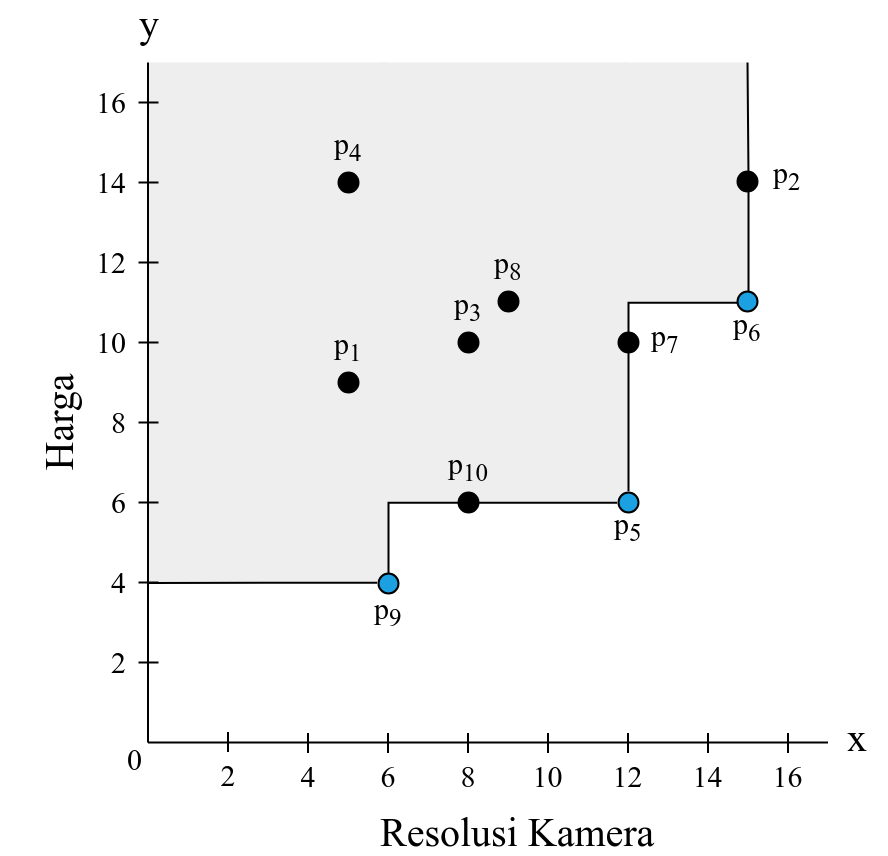
\includegraphics[width=6cm]{assets/img/bab2/skyline.png}
	\caption{Titik \textit{skyline} dari data produk pada Tabel \ref{tab:dataset}}
	\label{fig:skyline}
\end{figure}

\pagebreak
Berdasarkan Gambar \ref{fig:skyline}, produk \textit{smartphone} yang terbaik adalah $p_5$, $p_6$, dan $p_9$ karena tidak ada titik yang lebih baik dari titik-titik tersebut pada semua dimensi, sedangkan produk $p_{10}$ tidak dapat menjadi \textit{skyline} karena didominasi oleh produk $p_5$ pada dimensi $x$. Begitu juga produk $p_7$ yang didominasi $p_5$ pada dimensi $y$ dan produk $p_2$ yang didominasi $p_6$ pada dimensi $y$. Produk $p_5$, $p_6$, dan $p_9$ disebut dengan titik \textit{skyline} atau \textit{skyline point}.

Saat ini, komputasi \textit{skyline} telah banyak digunakan sebagai operator pengambil keputusan multikriteria dan perencanaan bisnis \cite{dynamic-skyline-2}. Ada beberapa pengembangan dari komputasi \textit{skyline}, seperti \textit{dynamic skyline} dan \textit{reverse skyline}.  

\section{Dominansi Dinamis}

\tab Berdasarkan definisi "\textit{Skyline}" yang telah dijelaskan pada sub-bagian sebelumnya, jika diberikan \textit{dataset} yang sama, maka hasil \textit{skyline} dari \textit{dataset} tersebut pasti akan selalu sama. Oleh karena itu, para ahli juga menyebut \textit{original skyline} sebagai \textit{static skyline} \cite{dynamic-skyline-2}.

Ada suatu kasus ketika perhitungan \textit{skyline} didasarkan pada titik kueri. Jika diberikan \textit{dataset} yang sama, namun titik kuerinya berbeda, maka hasil \textit{skyline}-nya pun berbeda tergantung pada titik kueri. \textit{Skyline} ini disebut dengan \textit{dynamic skyline} karena memiliki sifat dominansi dinamis. 

Diberikan \textit{dataset} produk $P$ dan \textit{dataset} pelanggan (preferensi pelanggan) $C$ yang setiap datanya direpresentasikan sebagai objek data $d$-dimensi dan hanya dapat menyimpan nilai numerik pada setiap dimensinya. Data produk dan pelanggan pada dimensi ke-$i$ dinotasikan sebagai $p^i$ dan $c^i$, $i \leq d$. Untuk menggambarkan objek data secara umum digunakan notasi $ob$.

\pagebreak
Suatu objek data $ob_1$ dikatakan mendominasi objek data $ob_2$ secara dinamis berdasarkan objek data $ob_3$, dinotasikan dengan $ob_1 \prec_{ob_3} ob_2$, jika nilai $ob_1$ dekat dengan $ob_3$ pada semua dimensi dan ada nilai $ob_1$ yang lebih dekat dengan $ob_3$ dibandingkan nilai $ob_2$ dengan $ob_3$ minimal pada satu dimensi. Secara matematika, relasi $ob_1 \prec_{ob_3} ob_2$ terbentuk jika dan hanya jika:
\begin{equation}\label{eq:syarat-dominansi-dinamis}
\begin{split}
\text{(a)} \tab |ob_3^i - ob_1^i| \leq |ob_3^i - ob_2^i|, \forall i \in [1, ..., d] \\
\text{(b)} \tab |ob_3^i - ob_1^i| < |ob_3^i - ob_2^i|, \exists i \in [1, ..., d]
\end{split}
\end{equation}

Pada Tabel \ref{tab:dataset}, diberikan contoh \textit{dataset} produk dan preferensi pelanggan. Berdasarkan preferensi pelanggan $c_1$, produk $p_1$ dikatakan mendominasi produk $p_2$, dinotasikan dengan $p_1 \prec_{c_1} p_2$, karena memenuhi kedua syarat dominansi dinamis yakni (a) $|c_1^1 - p_1^1| = |5-5| = 0 \leq |c_1^1 - p_2^1| = |5-15| = 10$ dan (b) $|c_1^2 - p_1^2| = |2-9| = 7 < |c_1^2 - p_2^2| = |2-14| = 12$.

\newcolumntype{C}{>{\centering\arraybackslash}p{2.5em}}
\begin{table}[H]
	\caption{Contoh \textit{dataset}\\(a) produk $P$ dan (b) preferensi pelanggan $C$ \label{tab:dataset}}
	\begin{subtable}{.5\linewidth}
		\small
		\centering
		\caption{}
		\begin{tabular}{|C|C|C|}
			\hline
			\textbf{id} & \textbf{dim1} & \textbf{dim2}\\ \hline \hline
			$p_1$ & 5 & 9\\ \hline
			$p_2$ & 15 & 14\\ \hline
			$p_3$ & 8 & 10\\ \hline
			$p_4$ & 5 & 14\\ \hline
			$p_5$ & 12 & 6\\ \hline
			$p_6$ & 15 & 11\\ \hline
			$p_7$ & 12 & 10\\ \hline
			$p_8$ & 9 & 11\\ \hline
			$p_9$ & 6 & 4\\ \hline
			$p_{10}$ & 8 & 6\\ \hline
		\end{tabular}
	\end{subtable}%
	\begin{subtable}{.5\linewidth}
		\small
		\centering
		\caption{}
		\begin{tabular}{|C|C|C|}
			\hline
			\textbf{id} & \textbf{dim1} & \textbf{dim2}\\ \hline \hline
			$c_1$ & 5 & 2\\ \hline
			$c_2$ & 8 & 10\\ \hline
			$c_3$ & 15 & 10\\ \hline
			$c_4$ & 9 & 7\\ \hline
			$c_5$ & 10 & 12\\ \hline
			$c_6$ & 12 & 14\\ \hline
			$c_7$ & 7 & 13\\ \hline
			$c_8$ & 15 & 8\\ \hline
			$c_9$ & 5 & 5\\ \hline
			$c_{10}$ & 10 & 5\\ \hline
		\end{tabular}
	\end{subtable} 
\end{table}

Sebaliknya, jika berdasarkan preferensi pelanggan $c_6$, maka produk $p_2$-lah yang mendominasi $p_1$, dinotasikan dengan $p_2 \prec_{c_6} p_1$, karena (a) $|c_6^1 - p_2^1| = |12-15| = 3 \leq |c_6^1 - p_1^1| = |12-5| = 7$ dan (b) $|c_6^2 - p_2^2| = |14-14| = 0 < |c_6^2 - p_1^2| = |14-9| = 5$. Dalam hal ini, preferensi pelanggan disebut dengan titik kueri karena dapat mempengaruhi sifat dominansi antar produk.

Mengambil contoh lain, produk $p_1$ tidak mendominasi $p_2$ berdasarkan pelanggan $c_3$ karena ada salah satu syarat dominansi dinamis yang tidak terpenuhi, (a) $|c_3^1 - p_1^1| = |15-5| = 10 \nleq |c_3^1 - p_2^1| = |15-15| = 0$ dan (b) $|c_3^2 - p_1^2| = |10-9| = 1 < |c_3^2 - p_2^2| = |10-14| = 4$. Produk $p_1$ dan $p_2$ dikatakan saling mendominasi berdasarkan pelanggan $c_2$.

\section{\textit{Dynamic Skyline}}
\tab Kueri \textit{dynamic skyline} dalam komputasi $k$-MPP digunakan untuk mencari produk terbaik dari sudut pandang pelanggan \cite{kmpp}, sehingga yang menjadi titik kueri adalah pelanggan. \textit{Dynamic skyline} \cite{dynamic-skyline} dari seorang pelanggan $c_1 \in C$, dinotasikan dengan $DSL(c_1)$, berisi semua produk $p_1 \in P$ yang tidak didominasi oleh produk lain $p_2 \in P$ berdasarkan preferensi pelanggan $c_1$, $p_2 \nprec_{c_1} p_1$.

\textit{Dynamic skyline} dapat dihitung menggunakan algoritme komputasi \textit{skyline} tradisional \cite{skyline}, yaitu mentransformasikan semua titik $p \in P$ ke ruang data baru dengan menganggap titik kueri $c$ sebagai titik asal dan jarak abolut titik $p$ ke $c$ digunakan sebagai fungsi pemetaan seperti yang ditunjukkan pada Gambar \ref{fig:dsl}. Fungsi pemetaan $f^i$ didefinisikan sebagai $f^i (p^i) = |c^i-p^i|$.

Menggunakan \textit{dataset} pada Tabel \ref{tab:dataset}, \textit{dynamic skyline} dari pelanggan $c_4$ adalah $DSL(c_4) = \{p_8, p_{10}\}$, karena produk tersebut tidak didominasi oleh produk lain berdasarkan preferensi pelanggan $c_4$. Berbeda halnya dengan $c_{10}$ yang memiliki hasil \textit{dynamic skyline} $DSL(c_{10}) = \{p_5, p_8, p_{10}\}$.

\begin{figure}[h]
	\centering
	\begin{subfigure}{.5\textwidth}
		\centering
		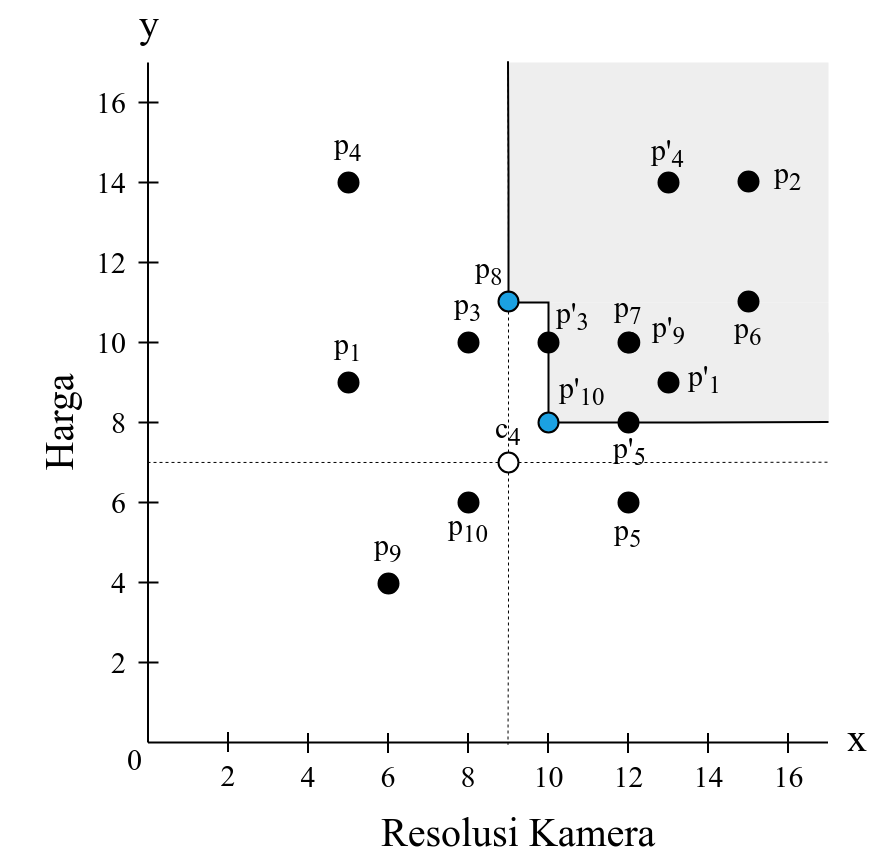
\includegraphics[height=5cm]{assets/img/bab2/dsl-1.png}
		\caption{}
	\end{subfigure}%
	\begin{subfigure}{.5\textwidth}
		\centering
		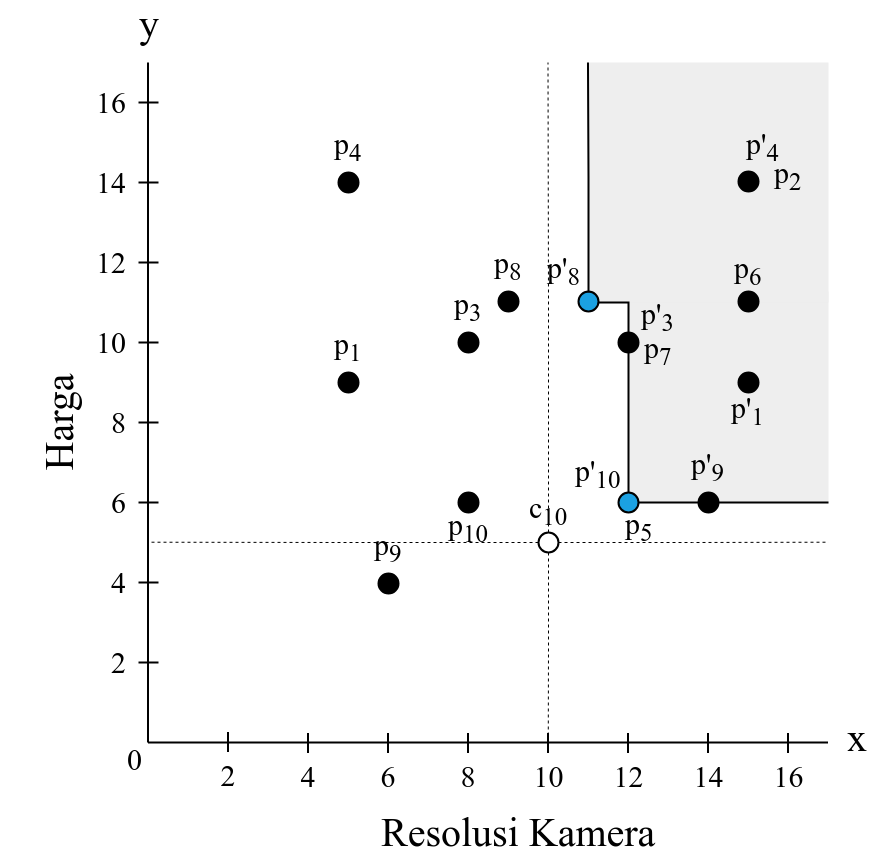
\includegraphics[height=5cm]{assets/img/bab2/dsl-2.png}
		\caption{}
	\end{subfigure}
	\caption{(a) Komputasi \textit{dynamic skyline} dari pelanggan $c_{4}$ dan (b) \textit{dynamic skyline} dari pelanggan $c_{10}$}
	\label{fig:dsl}
\end{figure}

\section{\textit{Reverse Skyline}}
\tab Dalam komputasi $k$-MPP, kueri \textit{reverse skyline} digunakan untuk mencari pelanggan potensial dari sudut pandang produsen \cite{kmpp}, sehingga yang menjadi titik kueri adalah produk. \textit{Reverse skyline} \cite{reverse-skyline} dari sebuah produk $p_1 \in
P$, dinotasikan dengan $RSL(p_1)$, berisi semua pelanggan $c \in C$ yang memiliki $p_1$ pada hasil \textit{dynamic skyline}-nya.

Ada beberapa tahapan yang harus dilakukan dalam komputasi \textit{reverse skyline} \cite{kmpp}. Pertama, menentukan \textit{orthant} dari produk, dinotasikan dengan $O$. Setiap produk $p$ memiliki $2^d$ \textit{orthant} pada data $d-$dimensi. Kedua, menghitung \textit{midpoint} atau titik tengah antara produk kueri dan produk lainnya, misalnya $p_1$ (sebagai titik kueri) dan $p_2$, dihitung menggunakan rumus berikut: 
\begin{equation} \label{eq:midpoint}
m_2^i = \frac{(p_1^i + p_2^i)}{2}
\end{equation}
Kemudian menentukan \textit{midpoint skyline} (juga dikenal sebagai \textit{mid-skyline} \cite{mid-skyline}) pada setiap \textit{orthant}.

Langkah ketiga, mengecek apakah pelanggan $c \in C$ didominasi oleh \textit{midpoint skyline} $m$ berdasarkan produk $p_1$ atau tidak. Pelanggan $c$ dikatakan didominasi oleh \textit{midpoint skyline} $m$ jika dan hanya jika:
\begin{equation}\label{eq:mid-skyline}
\begin{split}
\text{(a)} \tab |p_1^i - m^i| \leq |p_1^i - c^i|, \forall i \in [1, ..., d] \\
\text{(b)} \tab |p_1^i - m^i| < |p_1^i - c^i|, \exists i \in [1, ..., d]
\end{split}
\end{equation}

Apabila $c$ tidak didominasi oleh \textit{midpoint skyline} $m$ berdasarkan produk $p_1$, maka $c$ menjadi hasil dari \textit{reverse skyline} $p_1$, dinotasikan dengan $RSL(p_1)$. Untuk lebih jelasnya, komputasi \textit{reverse skyline} ditunjukkan pada Gambar \ref{fig:rsl}.

\begin{figure}[h]
	\centering
	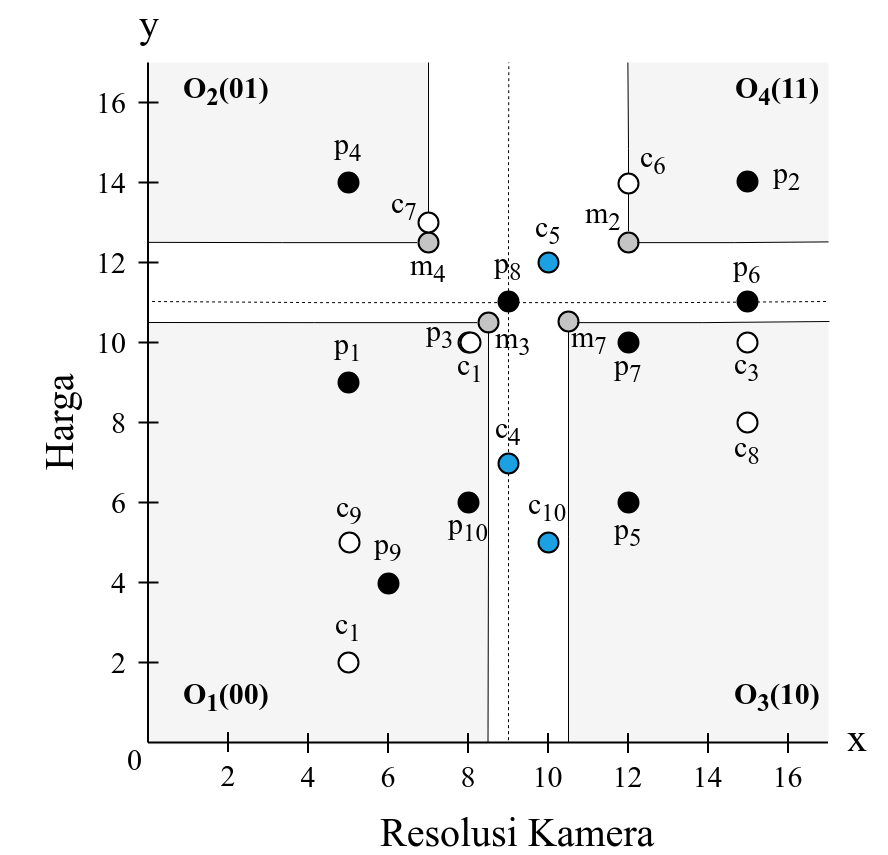
\includegraphics[height=6cm]{assets/img/bab2/rsl.png}
	\caption{Komputasi \textit{reverse skyline} dari produk $p_8$}
	\label{fig:rsl}
\end{figure}

Sebagai contoh, berdasarkan \textit{dataset} yang diberikan pada Tabel \ref{tab:dataset}, \textit{reverse skyline} dari produk $p_8$ adalah pelanggan $c_4$, $c_5$, dan $c_{10}$, dinotasikan dengan $RSL(p_8) = \{c_4, c_5, c_{10}\}$ karena masing-masing pelanggan tersebut memiliki $p_8$ pada hasil \textit{dynamic skyline}-nya.

\section{Kueri \textit{k-Most Promising Products} ($k$-MPP)}
\tab Kueri \textit{k-Most Promising Products} ($k$-MPP) adalah sebuah strategi pemilihan produk yang dikenalkan oleh Islam dan Liu dalam Tugas Akhirnya \cite{kmpp}.

\subsection{\textit{Uniform Product Adoption} (UPA)}
\tab \textit{Uniform Product Adoption} (UPA) mengasumsikan bahwa semua produk $p \in P$ yang muncul pada hasil \textit{dynamic skyline} pelanggan $c \in C$ akan saling berkompetisi satu sama lain untuk menarik pelanggan $c$, sehingga produk-produk tersebut memiliki probabilitas yang sama untuk dibeli oleh pelanggan $c$.

Probabilitas produk $p$ dibeli oleh pelanggan $c$, dinotasikan dengan $Pr(c, p|P)$ dapat dijelaskan oleh persamaan berikut:
\begin{equation}\label{eq:probability}
Pr(c, p|P) = \left\{
				\begin{array}{ll}
					\frac{1}{|DSL(c)|} & \text{if } p \in DSL(c)\\
					0 & \text{otherwise}\\
				\end{array}
				\right.
\end{equation}

Berdasarkan Persamaan \ref{eq:probability}, dapat dipastikan bahwa setiap produk yang muncul dalam $DSL(c)$ memiliki kesempatan yang sama untuk dipilih oleh pelanggan $c$. Sebaliknya, produk yang tidak muncul dalam $DSL(c)$ tidak memiliki kesempatan sama sekali untuk dipilih oleh $c$.

\pagebreak
Sebagai contoh menggunakan \textit{dataset} pada Tabel \ref{tab:dataset}, probabilitas produk $p_8$ dibeli oleh pelanggan $c_4$ adalah $Pr(c_4, p_8|P) = \frac{1}{|DSL(c_4)|} = \frac{1}{2}$, sedangkan probabilitas produk $p_8$ dibeli oleh pelanggan $c_{10}$ adalah $\frac{1}{|DSL(c_{10})|} = \frac{1}{3}$.

\subsubsection{\textit{Market Contribution}}
\tab \textit{Market contribution} atau kontribusi pasar sebuah produk $p \in P$ diukur dari total jumlah pelanggan yang mungkin lebih memilih membeli produk $p$ dibandingkan produk lain $p'$.

Asumsinya, jika seorang pelanggan memiliki dua produk atau lebih dalam hasil \textit{dynamic skyline}-nya, maka ia akan memberikan bobot yang sama pada produk-produk tersebut sebagaimana yang sudah dijelaskan pada Persamaan \ref{eq:probability}. Sehingga, kontribusi pasar sebuah produk dihitung dari hasil akumulasi bobot yang didapatkan dari semua pelanggan $c \in C$.

Kontribusi pasar produk $p$, dinotasikan dengan $E(C, p|P)$, diperoleh dengan mengakumulasikan probabilitas produk dari setiap pelanggan $c \in C$, sebagai berikut:\\
\begin{equation}\label{eq:market-contr}
E(C, p|P) = \sum_{\forall c \in C} Pr(c, p|P)
\end{equation}

Karena probabilitas produk $p$ dipilih oleh pelanggan yang tidak memiliki $p$ pada hasil \textit{dynamic skyline}-nya adalah nol (pada Persamaan \ref{eq:probability}), maka kita hanya perlu mengakumulasikan probabilitas produk dari setiap pelanggan $c$ pada hasil $RSL(p)$. Sehingga, Persamaan \ref{eq:market-contr} dapat disederhanakan menjadi:
\begin{equation}\label{eq:market-contr-rsl}
E(C, p|P) = \sum_{\forall c \in RSL(p)} Pr(c, p|P)
\end{equation}

\pagebreak
Sebagai contoh menggunakan \textit{dataset} pada Tabel \ref{tab:dataset}, kontribusi pasar dari produk $p_8$ adalah $E(C, p_8|P) = Pr(c_4, p_8|P) + Pr(c_5, p_8|P) + Pr(c_{10}, p_8|P) = \frac{1}{2} + 1 + \frac{1}{3} = \frac{11}{6}$ atau $1.833$.

Perhitungan kontribusi pasar juga dapat dilakukan pada sekumpulan produk atau \textit{subset} produk $P'$, dinotasikan dengan $E(C, P'|P)$, yang dijelaskan pada Persamaan \ref{eq:market-contr-subset}.
\begin{equation}\label{eq:market-contr-subset}
E(C, P'|P) = \sum_{\forall p \in P'} E(C, p|P)
\end{equation}

\subsection{Strategi Pemilihan Produk}
\tab Diberikan \textit{dataset} produk $P$, \textit{dataset} preferensi pelanggan $C$, dan bilangan bulat positif $k$ yang lebih kecil dari |P|. Kueri \textit{k-Most Promising Products} ($k$-MPP), dinotasikan oleh Persamaan \ref{eq:kmpp}, akan memilih \textit{subset} $k$ produk $P'$ dari $P$ yang memiliki kontribusi pasar lebih besar dibandingkan dengan \textit{subset} $k$ produk $P''$ dari $P$ yang lain \cite{kmpp}.
\begin{equation}\label{eq:kmpp}
k-MPP(P, C, k)
\end{equation}

Jika merangkum semua penjelasan di atas, langkah-langkah yang harus dilakukan untuk memproses kueri $k$-MPP adalah: (1) menghitung \textit{reverse skyline} dari setiap produk $p \in P$, (2) menghitung \textit{dynamic Skyline} dari setiap pelanggan $c \in RSL(p)$, dan (3) memilih \textit{k} produk dari $P$ yang memiliki kontribusi pasar terbesar.

\section{Python}
\tab Python adalah bahasa pemrograman tingkat tinggi, \textit{interpreted}, dan berorientasi objek yang didukung oleh struktur data \textit{built-in} tingkat tinggi dan semantik yang dinamis \cite{python}. Python dikembangkan oleh Guido van Rossum pada akhir 1980-an dan dikelola oleh \textit{Python Software Foundation}. Saat ini, Python sudah tersedia dalam dua versi, yakni 2.x dan 3.x.

Kelebihan bahasa pemrograman Python adalah pada keterbacaannya karena memiliki sintaksis yang sederhana, sehingga dapat mengurangi biaya pemeliharaan (\textit{maintenance}). Python mendukung banyak modul dan \textit{package}, serta memiliki banyak \textit{standard library} yang didistribusikan secara gratis. Selain itu, karena Python adalah bahasa \textit{interpreted}, Python tidak memakan biaya untuk kompilasi sehingga proses pengubahan, pengujian, dan debug menjadi lebih cepat.

Melakukan debug pada program Python sangatlah mudah karena tidak akan mengakibatkan \textit{segmentation fault}. Sebagai gantinya, ia akan menimbulkan \textit{Exception} apabila menemukan suatu \textit{error} atau kesalahan. Ketika program tidak menangkap \textit{Exception}, maka Python akan menampilkan \textit{stack trace} yang dapat digunakan untuk menganalisis dan memperbaiki kesalahan yang terjadi \cite{python}.

Dalam Tugas Akhir ini, bahasa pemrograman Python digunakan untuk mengimplementasikan struktur data dan algoritme pada sistem perangkat lunak yang akan dibangun. Python yang digunakan adalah versi 3.7.3.

\section{Flask}
\tab Flask adalah kerangka kerja web berbahasa Python yang sederhana, ringan, dan mudah dikembangkan, sehingga Flask kerap disebut dengan \textit{microframework}. Flask dibangun dari dua pustaka utama, yaitu Jinja \textit{template engine} dan Werkzeug WSGI \textit{toolkit}, serta memiliki lisensi BSD. Saat ini, Flask dikembangkan dan dikelola oleh \textit{Pallets team} dan kontributor komunitas \cite{flask}.

\pagebreak
Dalam Tugas Akhir ini, kerangka kerja Flask digunakan untuk mengimplementasikan aplikasi web dan layanan \textit{web server} yang digunakan pada Tugas Akhir ini karena ringan dan lebih mudah digunakan dibandingkan dengan \textit{framework} Python Django. Selain itu, Flask juga memiliki banyak dokumentasi dan tutorial yang dapat diikuti. Flask yang digunakan adalah versi 1.0.2.

\section{Vis.js}
\tab Vis.js adalah sebuah pustaka visualisasi berbasis web yang mudah digunakan, dapat menangani jumlah data yang besar secara dinamis, serta memungkinkan manipulasi dan interaksi dengan data. Pustaka ini terdiri dari komponen \textit{DataSet}, \textit{Timeline}, \textit{Network}, \textit{Graph2d}, dan \textit{Graph3d}. Pustaka yang dikembangkan oleh Almende B.V. ini berjalan dengan baik di sebagian besar peramban, seperti Chrome, Firefox, Opera, Safari, IE9 +, dan beberapa peramban seluler \cite{visjs}.

Dalam Tugas Akhir ini, pustaka Vis.js digunakan untuk memvisualisasikan data dalam bentuk lini masa atau \textit{timeline} pada sistem perangkat lunak yang akan dibangun. Vis.js yang digunakan adalah versi 4.21.0.